\documentclass{article}

\usepackage{ijcai09}
\usepackage{times}

\usepackage{algorithmic}
\usepackage{algorithm}

\usepackage{graphics} % for pdf, bitmapped graphics files
\usepackage{epsfig}
\usepackage{amsmath} % for postscript graphics files
\usepackage{subfigure}
\usepackage{fullpage}

\graphicspath{{../figures/}}

%\title{\LARGE \bf
%  Vision Based Obstacle Avoidance Using Neuro-Evolutionobot in Simulation
%}
\title{Vision Based Obstacle Avoidance Using Neuro-Evolution on a Differential Drive Robot in Simulation}

\author{ \parbox{3 in}{\centering Devin Koepl and Kevin Kemper\\
	\medskip
	\small{\textit{Dynamic Robotics Laboratory\\
	Oregon State University\\
	Corvallis, Oregon}}}
%	{\tt\small drl@oregonstate.com}}
}
	
\begin{document}
	\maketitle

	\begin{abstract}

		In this paper we present a vision feedback controller that uses an ensembles of compact artificial neural networks for obstacle avoidance on a simple robot in simulation. Our approach uses many simple artificial neural networks working in concert to select a heading at each time step based on the networks' confidence that the path chosen is clear.  that a collection of simple networks will be capable of better performance than any simple reflex controller we find and of similar performance to a single large artificial neural network provided sufficient training time, but will converge to a good solution faster than the large network.

	\end{abstract}


	\section{INTRODUCTION}
			
		Traditional approaches for robot obstacle avoidance rely many sensors.  This approach can be expensive to ruggedize and difficult to maintain such as LIDAR and sonar.  Many platforms already include cameras for high-level functions such as object recognition or tracking. An ideal solution would be to utilize only the camera for both reactionary sensing (such as object avoidance) and higher-level interactions.  One problem with this approach is that image data is difficult interpret - defining an obstacle verses a valid path is nontrivial.  In this paper we investigate a method for learning the classification of "safe" regions in an image to allow a simple robot to successfully navigate an environment.
		
		The approach we present in this paper improves the resolution of images that can be passed into an artificial neural network (ANN) ensemble learner used for robot obstacle avoidance by splitting the task of analyzing images amongst many small ANNs.  Conventional ANN image classification techniques use low resolution cameras or extensive down sampling to limit the complexity of solutions and make training times manageable.  However, these techniques waste a lot of the information that would be available in a higher resolution image, and require careful pre-processing to ensure that meaningful information is retained for input into the ANN.

		\begin{figure}[t]
			\begin{center}
				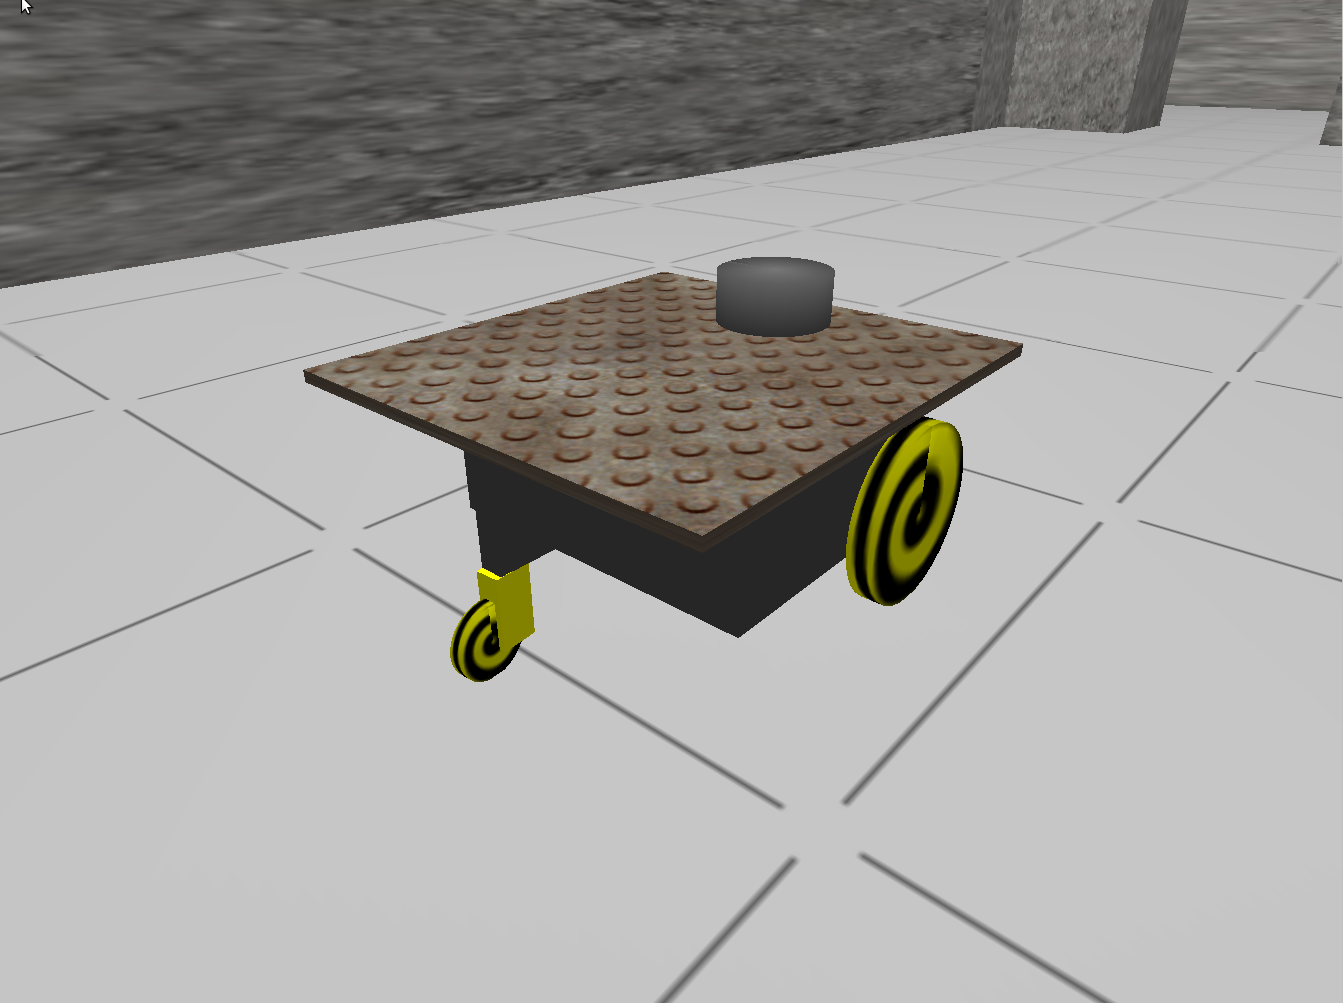
\includegraphics[width=\columnwidth]{robot1.png}
			\end{center}
			\caption{We test obstacle avoidance using a vision based ensemble neuro-evolutionary approach on a differential drive robot in simulation.}
			\label{robot}
		\end{figure}

		Our proposed approach overcomes the information loss and need for careful pre-processing associated with conventional ANN methods, but also avoids the complexity of an ANN that accepts full frame images as input by using a collection of simple neural networks that are easier to train than a single large network, but collectively are able to avoid obstacles as well as a single ANN implementation.  Instead of identifying and avoiding hazards in an entire image, each of our ANNs only needs to output an approximation of how safe it is to precede in the heading represented by a narrow column of the pre-processed image.  As an added benefit, we will be able to reuse the same collection of neural networks on all of the available headings, but for now we choose to use a separate pool of ANNs for each heading, because the narrow columns that the pre-processed image is divided into are identical in size and in this paper function, this reduces the number of ANNs that have to be stored, improves training time, and affords us room to experiment with larger ensemble sizes.

		We first show in simulation that our ensemble neural network algorithm is able to match the navigation commands of a human expert a high percentage of the time after limited training epochs.  In this paper we used an off-line neuro-evolutionary approach to demonstrate our ANN ensemble method.  Training data was generated by a human expert controlling the robot in the maze, and then our learner attempted to match the control commands of the human expert.  We then demonstrate the this approach on an unsupervised learner that is punished for contacting with obstacles.


	\section{BACKGROUND}

		Neural networks have been successfully applied to a wide range of problems including breast cancer diagnosis and stock market forcasts, but are particularly convenient for problem spaces with many continuous inputs \cite{Cheng1995} \cite{Chen2006}.  This makes them ideal for machine vision tasks where each pixel can act as one or more inputs to the network \cite{Pomerleau93_NNforVehicles},\cite{EgmontPetersen2002imageprocessingNN}.  Current cameras have millions of color pixels, for a neural network to make full use of this type of resolution it needs one or more inputs for each of the camera's pixels and perhaps thousands of hidden units.  Training and utilizing very large neural networks can be difficult because computations become expensive for the large number of training examples required to train them \cite{Giacinto2001}. Training examples also increases in complexity for neural networks with large numbers of inputs, more examples are required to adequately cover the input space, and training times increase. 
		
	One notable example of neural networks applied to vehicle control is ALVINN (Autonomous Land Vehicle In A Neural Network)\cite{Pomerleau93ALVINN} which is a neural network based lane-keeping system. Using simple color image pre-processing to create a grayscale input image and a 3 layer neural network architecture, ALVINN can learn, using back-propagation, the correct mapping from input image to output road location.  An interesting aspect of the ALVINN system is the method used to train it \cite{Pomerleau93_NNforVehicles}.  In this technique, called training "on-the-fly" the network is taught to imitate the driving reactions of a person.  As a person drives, the network is trained with back propagation using the latest video image as input the person's steering direction as the desired output.  This process works well for domains where there exists an expert but can fail to find general solutions unless the training data is very large, taking too much of the experts time.

		\begin{figure}[t]
			\begin{center}
				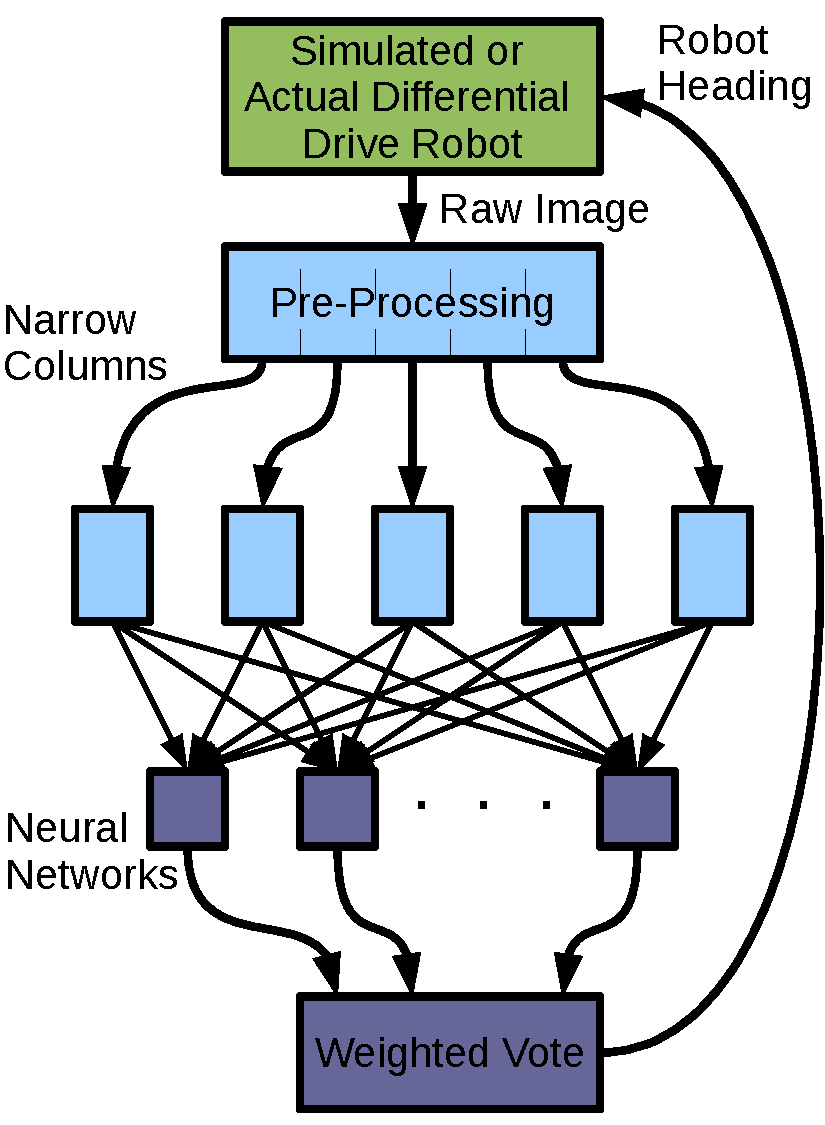
\includegraphics[width=\columnwidth]{block_diagram.pdf}
			\end{center}
			\caption{Block diagram of our artificial neural network control approach for obstacle avoidance on a differential drive robot.  Our ensemble of ANNs takes an image from our robot's forward facing camera as input, and outputs a heading that avoids obstacles.}
			\label{block_diagram}
		\end{figure}

		In another approach to using artificial neural networks for image processing, Baluja et.al. presented a method for dynamic relevance assessment using artificial neural networks \cite{Baluja97visionbasedfocus}. The network’s allocation of its limited representation capacity at the hidden layer is an indicator of what inputs it deems relevant to the task. By using only the hidden layer to predict the next input image, and comparing this prediction with the actual next image, they show that it is possible to estimate which inputs should be ignored and which should be attended. In deciding whether this approach is suitable to a new problem, there are two main criteria that must be considered. First, if expectation is to be used to remove distractions from the inputs, then given the current inputs, the activations of the relevant inputs in the next time step must be predictable. Additionally, the irrelevant inputs must either be unrelated to the task or be unpredictable.

	Other approaches to vehicle navigation using only optical flow.  Nelson argued that the flow field divergence represents a qualitative measurement which is useful for obstacle avoidance during visual navigation \cite{Nelson89ObstacleAvoidanceFlow}.  Coombs demonstrated a system that uses only real-time motion cues to wander while avoiding obstacles in a laboratory containing office furniture and robot and computing equipment \cite{Coombs98obstacleavoidanceflow}. The paper describes how flow, divergence of flow, and maximal flows are computed in real-time to provide the robot’s sense of space, and how steering, collision detection, and camera gaze control together accomplish safe wandering.  Using these concepts as preprocessing for the inputs to the artificial neural network, it may be possible to gain the benefits of both.

		The final concept we pan to utilize revolves around ensemble methods.  It has been shown that robustness of ANN learning can be improved by ensemble methods \cite{Hansen1990}.  Considerable work has been done to investigate the potential of such methods for a variety of applications such as function approximation \cite{Hansen1990}, estimating chlorophyll concentration in coastal waters with satellite data \cite{Slade03_enn_sat} and currency identification \cite{Debnath09_enn_money}.  When ANNs are grouped together in an ensemble their individual errors can be taken care of by considering the output of all ANNs in the ensemble, provided that ANNs make independent errors.  Our motivation for this work presented in this paper comes from the success of these investigations at increasing the robustness of ANN learning, provided that ANNs in an ensemble do not make identical errors, without increasing the complexity of the individual learners in the ensemble.

	\section{PROBLEM DOMAIN}

		Our proposed approach uses eight pools of simple single hidden layer ANNs that accept a narrow column of the pre-processed image captured by our robot's camera, and return a confidence that the small image represents a safe direction to precede in, as shown in Fig. \ref{block_diagram}.  At each time step an image is captured by our robot's camera, such as the image shown in Fig. \ref{robot_cam}, and our robot's heading is chosen by a weighted vote between the ANNs.  Each pool of ANNs is used on its column of the pre-processed image, and casts a vote based on its confidence that the direction represented by the column, with a weight reflective of its accuracy during training.

		\begin{figure}[t]
			\begin{center}
				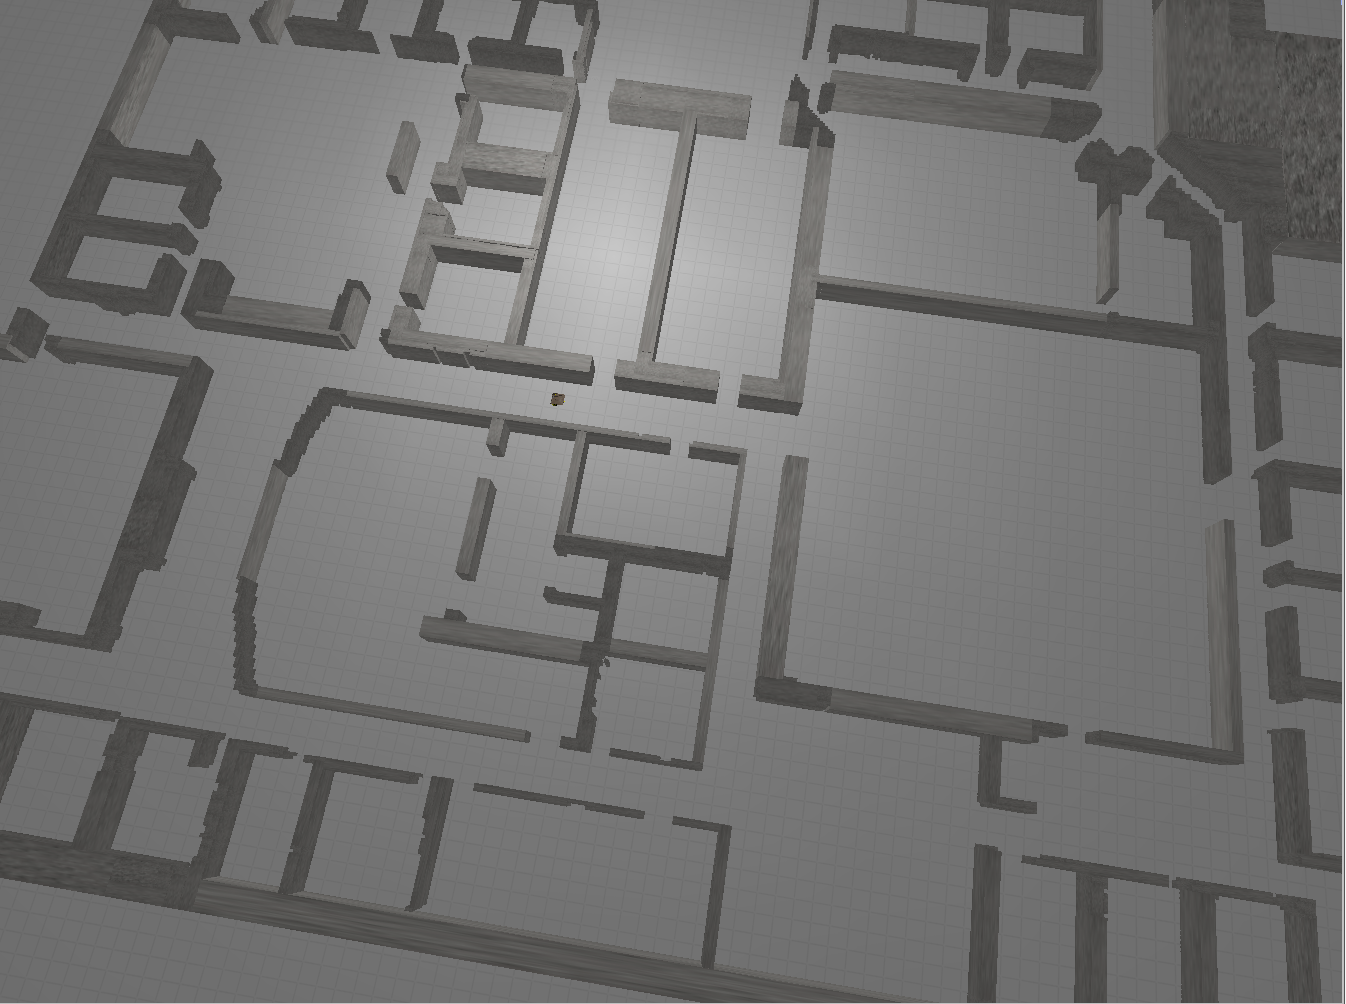
\includegraphics[width=\columnwidth]{world.png}
			\end{center}
			\caption{We test our ensemble artificial neural network solution in a complex maze world.}
			\label{world}
		\end{figure}

		Our approach uses offline neuro-evolution to create a collection of ANNs capable of navigating our simulated robot through its environment while colliding with as few obstacles as possible.  Training begins with a collection of neural networks with random weights and uniform voting power, and will consist of releasing the simulated robot in a training environment.  Large penalties will be assessed after collisions with the environment based on networks' confidences in the direction that led to the collision, and smaller penalties will be assessed to the neural networks that expressed confidence in the directions that led up to the collision.  Rewards will be given for confidence in directions that do not lead to collisions.  We would also like to investigate more omniscience rewards that consider our robot's proximity to hazards and assess rewards for maintaining its distance from hazards.  After each timestep, the poorest performing neural networks will be discarded, and the best performing neural networks will be duplicated with some mutations and an initial voting power that places them in the lower-middle of the collection, maintaining the size of the neural network collection. 

		We use Open Dynamics Engine (ODE) to simulate our robot in its environment.  ODE handles any physics that are required and any collisions that occur between our robot and the environment.  In addition to ODE we also use Robot Operating System (ROS).  ROS handles the shared memory that allows us to pass images and control commands between our simulation and controller, and includes 3D visualization environments, RVIZ and Gazebo, which we use to generate and capture images for input into our controller.  We use OpenCV for our pre-processing routine, as this library includes functions for matrix operations, edge and flow detection.  The controller we test in this paper was implemented in C++ such that the necessary ROS and OpenCV libaries could be easily included.  Future controllers in our final paper will be create similarly, as executables called by ROS and compiled from C++ code.

			\begin{figure}[tight]
				\subfigure[Screenshot of our artificial neural network navigating our differential drive robot through the maze we tested it in.]{
					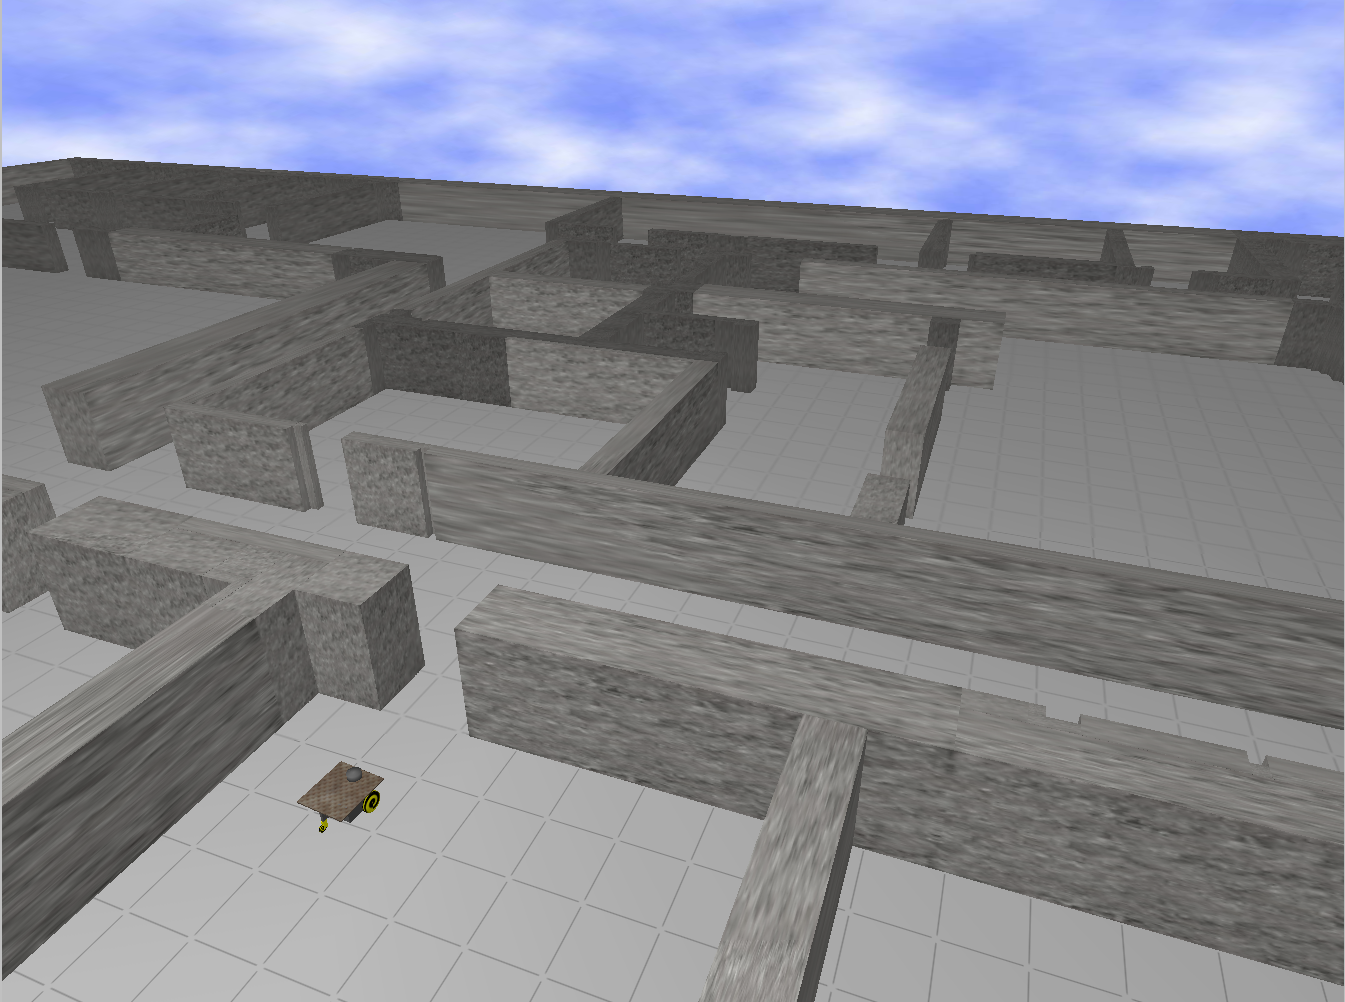
\includegraphics[width=0.46\columnwidth]{robot2.png}
					\label{robot_in_maze}
				}
				\subfigure[This is the image captured by our robot's camera corresponding the the instant that the screenshot to the left was taken.  Images such as this one are passed into our pre-processing algorithm and then into our ANN ensemble.]{
					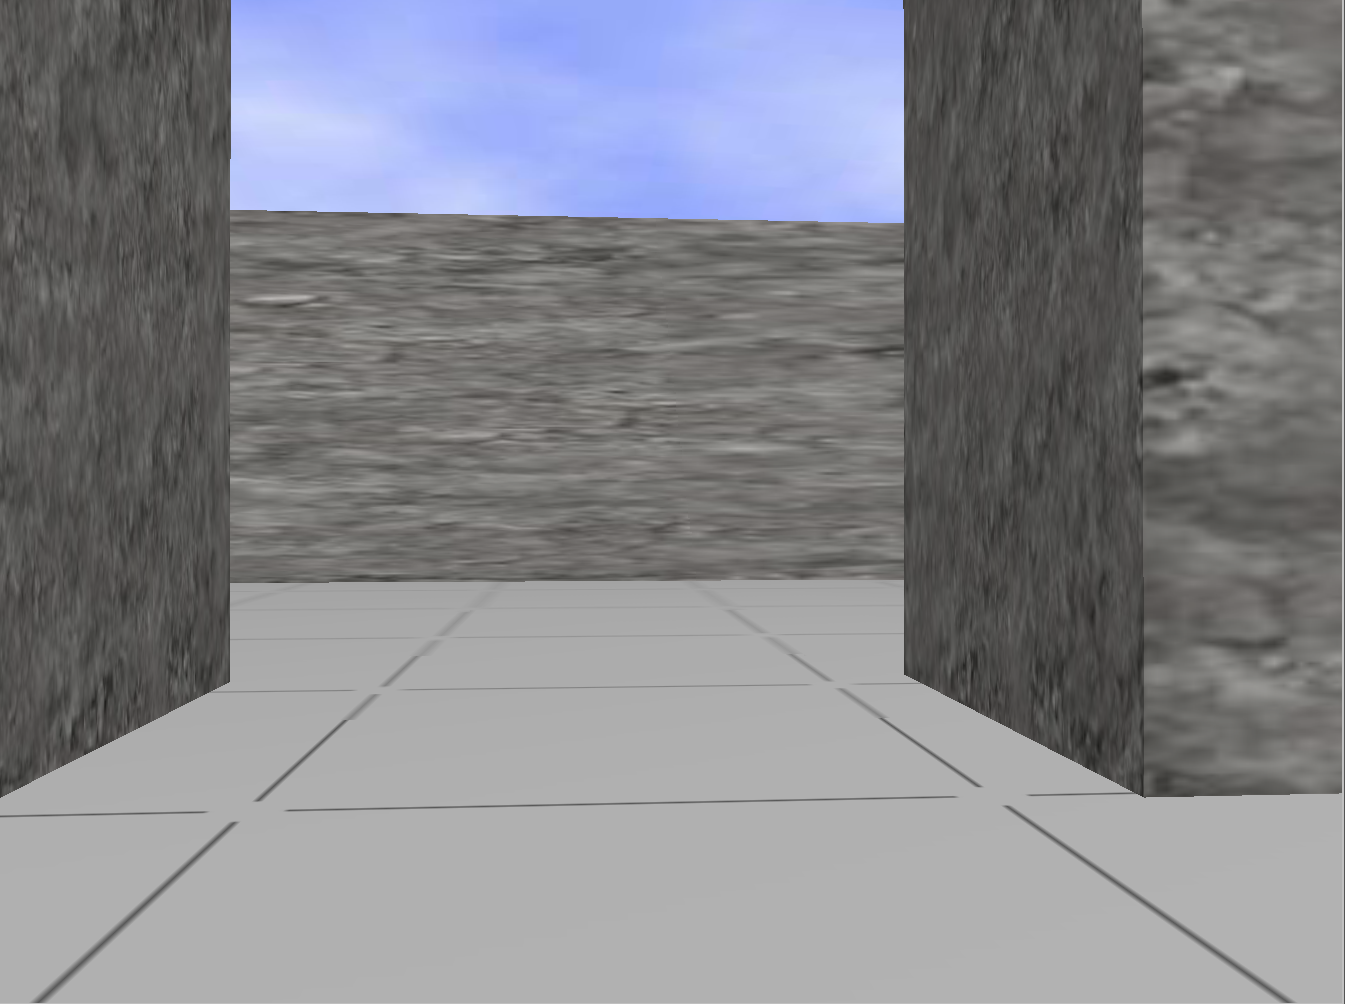
\includegraphics[width=0.46\columnwidth]{robot_cam.png}
					\label{robot_cam}
				}
				\caption{Images taken of our robot in the maze, and by our robot's camera at the same instant.}
			\end{figure}

		Our robot travels at a constant forward speed, and is not able to adjust its speed, it is only able to steer.  Although our robot's environment is continuous, it is only able to update its heading at regular fixed timestep intervals.  This simulates the hardware limitations of a mobile robot driving in the real world, where image capture and computation are not instantaneous.  ODE allows us to simulate realistic differential drive robot physics, leaving the option of more complex environments with changes in ground surface height available.  Using a realistic physics simulation should also make the controllers that our ANN ensemble learns more transferable to an actual robot, which will be subject to similar dynamic constraints.

\section{EXPERIMENTS}
\label{sec:ex}

	In this paper we first demonstrate how our ensemble neural network approach can be used with online expert learning for obstacle avoidance in a complex maze, shown in Fig. \ref{world}. We use an expert human driver to generate training data by navigating our robot through the maze using keyboard commands that correspond to actions available to our neural network.  Training data consists of raw images captured our robots camera, and the keyboard commands.  The grade for a learner is based on the average difference between the expert and the neural-network command.

	The second experiment consisted of of the robot in Fig. \ref{robot_in_maze} learning to navigate the maze in an unsupervised fashion.  In the implementation of our unsupervised learning algorithm it was arbitrarily chosen that a learning episode consist of testing one hundred ensemble neural network controllers over a period of one thousand images each from our robot's camera.  We added a simple bump sensor to the top plate of our robot that allowed a low level controller to temporarily lock out the ensemble neural network controller while it moved the robot  away from the object it collided with, this prevented our robot from becoming stuck against a wall during unsupervised training.  This low-level controller was important to our specific implementation, because we restrict our controller to steering the robot, but not adjusting its forward velocity.  During our unsupervised learning experiment our robot simulation was never reset, instead new ensemble neural network controllers simply picked up where the last controller left off.  We chose this implementation because we felt it best simulated how unsupervised learning might be implemented on an actual robot where resetting the system state may be inconvenient or impossible.

	For both tasks, the same learning approach outlined in Alg. \ref{alg:evo} is used.  The difference is in the cost function to grade the mutated networks.


%	In our final paper, we will compare our collective neural network approach to a single neural network solution and controllers that we devise in simulation.  We will generate a training environment, and several test environments with varying levels of complexity which we will simulate in ODE.  We will plot performance versus the number of training epochs for the controllers in several test environments.  Performance will be measured as the probability that a collision occurs during a timestep in a test environment.  This measurement will be taken by setting a robot loose in the environment for a large fixed number of timesteps.  When a collision occurs the robot will be reset to a random position in the environment.  After all of the timesteps are completed the probability that a collision occurs in a timestep is just the total number of collisions that occurred divided by the length of the test.

%	For now we demonstrate an expert system as a proof-of-concept for our ANN ensemble method.  Implementing additional controllers and learning algorithms should now be straight forward, since we already have a simulation platform, and mechanism for interfacing our controllers with our simulation.

\begin{algorithm}[t, tight]
\caption{Evolutionary trial}
\label{alg:evo}
\begin{algorithmic}

	\STATE Generate 8 random populations of neural networks

	\FOR {50 episodes}
		
		\FOR {Each population}
			\STATE $chosen \gets$ best or random using $\epsilon$-greedy.
			\STATE $mutant \gets mutate(chosen)$
		\ENDFOR
				
		\FOR {100 images}
		
			\STATE Split image into 8 slices
			
			\FOR {Each slice}
				\STATE Evaluate slice with corresponding mutant
				\STATE $grade \gets grade + punisment$
			\ENDFOR
			
		\ENDFOR

		\FOR {Each population}		
			\IF{$grade < worst(population)$}
				\STATE Replace worst in the population with the mutant.
			\ENDIF
		\ENDFOR

	\ENDFOR
\end{algorithmic}
\end{algorithm}



%		We will compare our neural network solutions against simple reflex agent controllers of our own design.  These controllers will include a controller that directs our robot to drive in the direction of the lowest absolute optical flows, a controller that directs our robot to drive in the direction of the fewest edges, and any other controllers that we find to test against.  We suspect that the single and collective neural network solutions will be able to outperform any simple reflex agent we devise to control our robot, given sufficient training time.  The simple reflex agents will be able to avoid obstacles in specific environments, but will not be able to avoid obstacles in other environments.  For example, the simple reflex agent that drives towards lower concentrations of edges will perform poorly in environments with a textured ground surface and smooth solid colored objects.




\section{Results}

		\begin{figure}[t, tight]
			\vspace{-6pt}
			\subfigure[Initial untrained output given the input frame.]{
				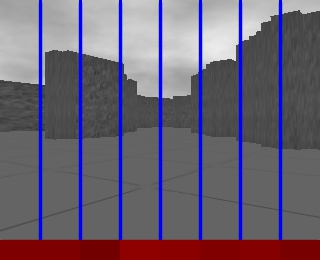
\includegraphics[width=0.46\columnwidth]{output_0.jpg}
				\label{fig:ex_io0}
			}
			\subfigure[First set of mutations applied to the weights.]{
				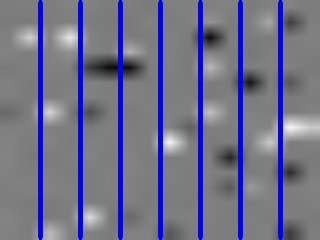
\includegraphics[width=0.46\columnwidth]{weights_0.jpg}
				\label{fig:ex_w0}
			}

			\subfigure[Output from trained networks.]{
				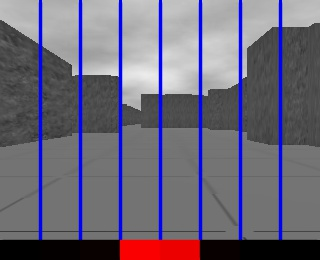
\includegraphics[width=0.46\columnwidth]{output_end.jpg}
				\label{fig:ex_ioEnd}
			}
			\subfigure[Weights of trained networks, there is no obvious pattern.]{
				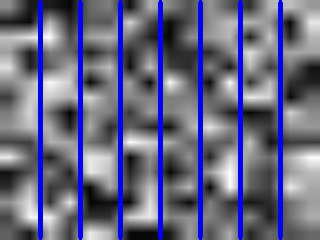
\includegraphics[width=0.46\columnwidth]{weights_end.jpg}
				\label{fig:ex_wEnd}
			}
% I'm trying to be ambiguous here for now
			\label{fig:exOutput}
			\vspace{-6pt}
			\caption{Example of the response from each network given an image.  The blue line indicate the boundaries between the image segments given to a neural network.  The red box under each segment indicates the networks response to the input image segment.  The intensity of red indicates the a strong response.  For the weight images, gray is a weight of 0 with darker shades indicating negative and lighter positive.}
			\vspace{-6pt}
		\end{figure}

		\begin{figure}[tight]
			\begin{center}
				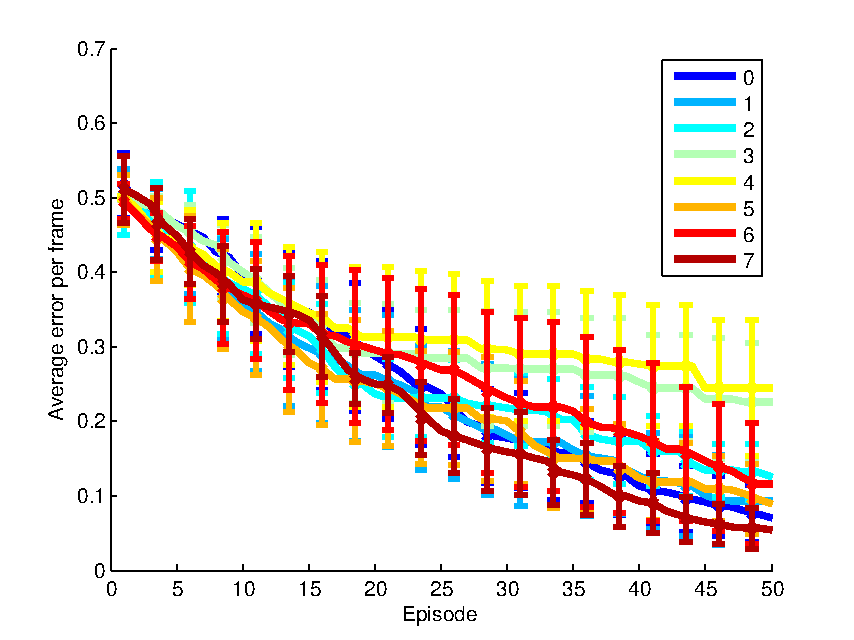
\includegraphics[width=1.1\columnwidth]{data.pdf}
			\end{center}
			\vspace{-6pt}
			\caption{Training results averaged over 10 trials.  Each graph indicates the performance per slice of frame.  Slice zero represents the left most slice of the image with slices evenly space from there.}
			\vspace{-6pt}
			\label{fig:graph}
		\end{figure}


		The method detailed in section \ref{sec:ex} was tested over a set of 855 image and command pairs.  Each image is flattened into grayscale and then down-sampled to 16x16 pixels and sliced into 8 equal columns (illustrated in Fig. \ref{fig:exOutput}).  Each slice is then fed into an ANN following algorithm \ref{alg:evo}.  Each learning episode takes place over 50 images with one trial lasting for 50 episodes.  A representative run is shown in Fig. \ref{fig:exOutput} which shows the state of the weights and an example output after the first set of mutations (Figs. \ref{fig:ex_io0},\ref{fig:ex_w0}) and after 50 episodes (Figs. \ref{fig:ex_ioEnd},\ref{fig:ex_wEnd}).  One thing to note is that for the current training method, the weights do not seem to converge to some pattern.  It should be expected that a generalized solution should show spots in the weights indicating important locations (e.g. near the lower part of the image).  For now, the problem is likely in our training set.

		A graph indicating the learning rates of the ANN populations associated with an image slice is given in Fig. \ref{fig:graph}.  Each population reduces the error in matching its output against the example command over the each trial.  Given more episodes it is possible to reduce the error to almost zero but again, the current training set does not capture enough situations to allow for a general solution.  One thing of interest is how the ANN associated with the center image slices tend to learn at a slower rate than others.  This could be explained by the fact that for most of the example commands the robot is set to go forward (i.e. high activation in the center of the image).  When the examples do show a turn, it is often a "soft" turn where the robot does not need to turn quickly.  This keeps the average activation near the center of the images.
		
		We then implemented our neuroevolutionary algorithm in an unsupervised system using 100 frames for each learning episode. The ensemble network demonstrated on our simulated robot often discovered good control policies in fewer than twenty learning episodes, as shown in \ref{fig:unsupervised_results}.  However, depending on how we setup our cost function, the ANNs that achieved the lowest penalties tended to spin the robot in tight circles.  Spinning in an open space ensures that no penalties will be incurred for collisions, and is difficult to penalize without discouraging turning.  One interesting note is how the penalty in Fig. \ref{fig:unsupervised_results} initially increases in general.  This might be explained by the fact that when a trial begins the robot is set in the center of a room.  After early episodes complete the robot will likely end up near a wall or corner, increasing the potential of the learner to collide and incur a penalty.
	
	\section{Conclusions and Future Work}

		For now we demonstrate our unique approach for obstacle avoidance on a robot with only visual feedback using an expert system and unsupervised learning as a proof-of-concept for our approach and simulation platform.  Our ensemble ANN method converges quickly with the expert, learning to match the commands of a human expert given the same forward-facing camera view as the human driver.  We then tested the ensemble in an unsupervised method using simple bump sensors with reactionary low-level control to keep the robot from getting stuck.  Already the neural network solutions learned by our approach should transfer easily to a physical platform, and provided that teleoperation of the robot would be available, the supervised learning we implemented in simulation would still be possible.

		By dividing images captured by our robot into narrow columns, we reduce the complexity of the ANNs needed to process them.  This is a good thing. Smaller neural networks are faster to train and less computationally expensive to evaluate.  For example, a single ANN accepting full frame images as input, has to learn to recognize hazards across the full field of view of the camera, which ends up being many times the number of weights to learn.
		
		Although our unsupervised learning implementation learned to optimize the cost functions we tested, it was difficult to design a cost function that simultaneously encouraged our robot to explore, and yet still avoid collisions with the environment.  When our controllers where not penalized for turns, the solution that optimized the cost function was to steer the robot in tight circles.  This behavior ensured that our robot would not collide with any obstacles, and while perhaps not all that useful or interesting, it demonstrates our approache's ability to find optimal solutions in a complex learning environment.  However, we were also interested in finding a cost function that would encourage more sophisticated behaviors, so we tested several cost functions that penalized turns with varying results.  In the best case, our learner came up with controllers that circled about the outside of a room, but we were unable to concieve a cost function that would balance risky exploratory behaviors, such as navigating narrow doorways and hallways, with safe behaviors like circling in an open room.  Through these experiments it became apparent that some higher level objectives such as reaching a desired destination or exploring as much of the world as possible were needed for our approach to learn more interesting control policies.

		\begin{figure} [t]
			\vspace{-6pt}
			\begin{center}
				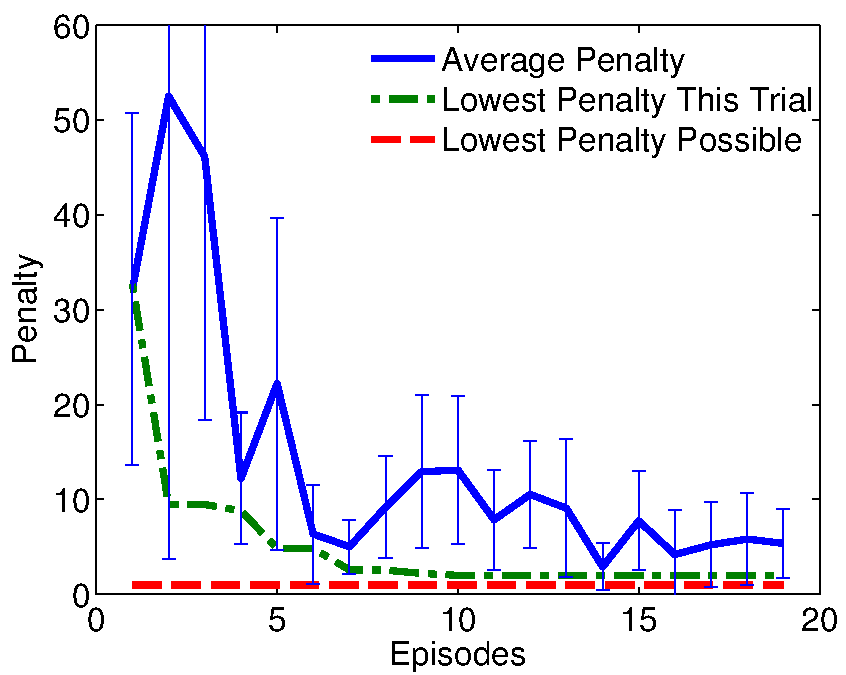
\includegraphics[width=\columnwidth]{unsupervised_results.pdf}
			\end{center}
			\vspace{-6pt}
			\caption{Results from our neuro evolutionary approach implemented as an unsupervised learner averaged over 86 trials.  Error bars represent one half standard deviation from top to bottom.  In addition to the average penalty, we also plot the lowest possible penalty, and the lowest penalty seen on a specific trial.}
			\vspace{-6pt}
			\label{fig:unsupervised_results}
		\end{figure}

		In the future we would like to investigate different reward structures and pre-processing algorithms.  We believe that the performance of either a single neural network solution or our collective neural network solution could be improved by giving rewards for increasing the distance between our robot and obstacles in the environment and assessing penalties for coming close to colliding.  In addition to our edge and flow detection algorithms, we would also like to test other algorithms as part of our pre-processing routine.  For example, we suspect that we can improve the performance of either of the neural network controllers we are testing by averaging several successive images together at each time step.

		To further extend this work we would like to tune our neural network ensemble method for better performance in more complex environments.  The maze world presented in this paper consisted of a flat rigid plane with high vertical walls, and did not include variations in floor, wall, or sky texture.  Walls were for the most part of uniform height, and the ground surface height was constant.  For our approach to be useful in real world environments where the diversity of hazards will be greater, it must first be trained in simulation to avoid a greater variety of hazards.  Our robot's obstacle avoidance goal could also be augmented with other goals such as navigating to a specific location in the world or a particular object.  
	
		Eventually we would like to demonstrate our neural network ensemble approach on an actual robot.  The platform we simulate could be easily realized as a physical system that should closely match the dynamics of our simulated robot.

	\vspace{-6pt}

	\bibliographystyle{named}
	\bibliography{../papers/me537}

\end{document}
